\chapter{Probabilidad, información y entropía}

\lectureoverview{La mecánica estadística comienza donde las leyes microscópicas se encuentran con el conocimiento incompleto. Primero damos precisión al concepto de probabilidad y luego preguntamos cómo el propio movimiento determinista asigna probabilidades, cómo las leyes de conservación dividen el espacio de estados y por qué la dinámica que conserva la información conduce de manera natural a la entropía. Las leyes primera y cero solo entran en escena una vez establecida esta estructura.}

\section{¿Por qué estudiar mecánica estadística?}

A veces se describe la mecánica estadística como física antigua. Esa descripción pasa por alto lo esencial. Es anterior a la modernidad, moderna y probablemente seguirá siendo útil en cualquier física posmoderna que suceda a las teorías que conocemos. Los modelos particulares aparecen y desaparecen; la segunda ley de la termodinámica ha sobrevivido repetidamente como guía. Siempre que una descripción propuesta de la naturaleza parezca generar orden de la nada, borrar información de forma fundamental o hacer que un sistema cerrado evolucione hacia un estado anormalmente simple, la segunda ley nos advierte que se ha dejado algo fuera.

El tema puede parecer menos fascinante que una partícula recién descubierta, pero es al menos igual de profundo y mucho más general. Los gases, los líquidos, los sólidos, la radiación, los agujeros negros, la información y los campos cuánticos requieren razonamiento estadístico. De hecho, no se podría entender la maquinaria experimental utilizada para descubrir partículas sin él. Por eso generaciones de físicos destacados dominaron la mecánica estadística incluso cuando su trabajo principal se desarrollaba en otros campos: el tema es útil, pero también posee una belleza excepcional.

Para ver por qué hace falta, partamos del ideal que ofrece la mecánica. Un sistema cerrado es el universo entero que se considera o un subsistema lo bastante aislado como para que su entorno no influya en él. Si conocemos su condición inicial y su ley de evolución, la mecánica clásica ofrece una predicción completa. La mecánica cuántica modifica lo que se puede predecir, pero también tiene un estado definido con precisión y una ley que predice la información máxima que permite la teoría.

Hay una diferencia profunda entre predecir en principio y comprender de manera útil. Una lista con la posición y la velocidad de cada molécula de esta habitación sería extraordinariamente larga, cambiaría casi de inmediato y respondería pocas de las preguntas que realmente nos interesan. Por tanto, las leyes microscópicas exactas pueden ser perfectamente predictivas y, al mismo tiempo, inútiles en la práctica.

La mecánica estadística es la teoría de la probabilidad aplicada a esta situación física. Se vuelve necesaria cuando no se conoce la condición inicial con exactitud perfecta, cuando la ley solo se conoce de manera aproximada, cuando el sistema es abierto o, sencillamente, cuando hay demasiadas variables microscópicas para seguirles la pista. Nada de esto implica que las predicciones sean poco precisas. A menudo, los números grandes hacen que las predicciones estadísticas sean extraordinariamente precisas.

Consideremos una caja aislada con gas. No podemos predecir la trayectoria de cada molécula, pero unos pocos datos macroscópicos nos permiten predecir con gran precisión la presión, la energía y muchas otras magnitudes macroscópicas. Lo que sigue siendo incierto son las fluctuaciones. En un momento impredecible, una región pequeña puede contener más moléculas que el promedio, mientras que otra contiene menos. Ese suceso se encuentra en la cola de una distribución de probabilidad: es improbable, pero no está prohibido. Podemos calcular con qué frecuencia deberían producirse tales fluctuaciones sin predecir el instante en que ocurrirá una en particular.

El lanzamiento de una moneda muestra la misma distinción. En mil millones de lanzamientos justos, los números de caras y cruces serán casi iguales. Si lanzamos la moneda suficientes veces, tarde o temprano aparecerá una larga racha de caras, pero la teoría de la probabilidad predice su frecuencia, no de antemano cuándo ocurrirá. La mecánica estadística está pensada para sistemas cuyos elementos son demasiado pequeños, demasiado numerosos o ambas cosas.

El curso desarrollará las leyes y sus aplicaciones a la materia. El tema recompensa el estudio reiterado: uno lo aprende, olvida algunas partes y vuelve a aprenderlo con una comprensión más profunda de cuáles ideas son fundamentales. Empezamos con la idea que rige todo lo que sigue.

\section{La probabilidad como lenguaje primitivo}

La razón por la que funciona la probabilidad no es algo que explique el propio cálculo de probabilidades. Una predicción probabilística puede fallar en un ensayo concreto; eso es lo que significa que un resultado sea posible, pero improbable. La teoría nos dice cómo se distribuyen las excepciones. No las elimina. Por eso tomamos la probabilidad como concepto primitivo y enunciamos las reglas que obedece.

\subsection{Estados y normalización}

Sea \(i\) la etiqueta de un resultado posible o de un estado posible de un sistema. Para una moneda, \(i\) puede representar cara o cruz. Para un dado, puede tomar valores desde \(1\) hasta \(6\). Para dos dados, un par de índices registra las dos caras. Empezamos con un espacio de estados discreto y finito,
\begin{equation}
 i=1,\ldots,N,
\end{equation}
y más adelante pasaremos a espacios con infinitos estados y a espacios con un continuo de estados.

La ignorancia no significa que el sistema carezca de estado. Significa que no sabemos cuál es su estado, así que asignamos una probabilidad \(p_i\) a cada posibilidad. Las reglas básicas son
\begin{align}
 p_i &\geq 0, \label{eq:sm1-prob-positive}\\
 \sum_{i=1}^{N}p_i &=1. \label{eq:sm1-prob-normalization}
\end{align}
Las alternativas son mutuamente excluyentes y exhaustivas: ocurre exactamente una de ellas. Aquí las probabilidades negativas no tienen cabida, y la suma es uno porque necesariamente ocurre algún resultado permitido.

\subsection{Frecuencia y ley de los grandes números}

La probabilidad se relaciona con el experimento mediante ensayos repetidos. Supongamos que se realiza \(N_{\mathrm{trials}}\) veces el mismo experimento y que \(N(i)\) es el número de ensayos que producen el resultado \(i\). Entonces, la interpretación frecuencial es
\begin{equation}
 p_i=
 \lim_{N_{\mathrm{trials}}\to\infty}
 \frac{N(i)}{N_{\mathrm{trials}}}.
 \label{eq:sm1-frequency}
\end{equation}
Se trata de una hipótesis física expresada mediante un límite ideal. Ningún laboratorio realiza infinitos experimentos. La afirmación es que, con suficientes ensayos, la razón se aproxima lo bastante a \(p_i\) para la predicción que se pretende hacer. Las muestras finitas fluctúan en torno al valor límite.

\subsection{Promedios}

Ahora asignemos un número \(f(i)\) a cada estado. Puede ser la energía, el momento u otra magnitud que queramos medir. Su valor esperado es
\begin{equation}
 \langle f\rangle=\sum_i f(i)p_i.
 \label{eq:sm1-expectation}
\end{equation}
La notación de corchetes resulta cómoda incluso fuera de la mecánica cuántica. En términos de frecuencias, el mismo promedio es
\begin{equation}
 \langle f\rangle
 =
 \lim_{N_{\mathrm{trials}}\to\infty}
 \frac{1}{N_{\mathrm{trials}}}
 \sum_i f(i)N(i).
 \label{eq:sm1-frequency-average}
\end{equation}

Para una moneda, definamos
\begin{equation}
 f(\mathrm{H})=+1,
 \qquad
 f(\mathrm{T})=-1.
\end{equation}
Si cara y cruz tienen cada una probabilidad \(1/2\), entonces
\begin{equation}
 \langle f\rangle
 =(+1)\frac12+(-1)\frac12=0.
\end{equation}
El promedio no tiene por qué ser un resultado posible. La moneda nunca cae en cero; el cero resume la distribución de sus dos valores posibles.

Esta breve digresión fija el vocabulario que se empleará en todo el tema: estados, probabilidades, frecuencias y valores esperados.

\section{Tres maneras de asignar probabilidades}

\subsection{Simetría}

¿Por qué solemos asignar probabilidades iguales a las dos caras de una moneda? La primera respuesta es la simetría. Al darle la vuelta a una moneda casi ideal se intercambian cara y cruz sin cambiar el experimento. En ese caso, no hay ninguna razón física para favorecer un resultado sobre el otro. Una marca o imperfección real introduce un pequeño sesgo, pero el modelo simétrico representa el experimento que se pretende describir:
\begin{equation}
 p(\mathrm{H})=p(\mathrm{T})=\frac12.
\end{equation}

El mismo razonamiento asigna probabilidad \(1/6\) a cada cara de un dado simétrico. En general, se asignan probabilidades iguales a las configuraciones relacionadas por una simetría, salvo que alguna información adicional rompa esa simetría.

\subsection{Experimento}

Un dado deforme no tiene ninguna simetría que intercambie sus seis caras. En ese caso, la simetría por sí sola no da una respuesta. Puede que tengamos un modelo mecánico más profundo que prediga el sesgo, pero, si no disponemos de él, el procedimiento honesto es experimental: lanzar el dado muchas veces, registrar las frecuencias, esperar a que se estabilicen y utilizar la tabla de probabilidades resultante en predicciones posteriores.

La simetría y el experimento no son definiciones que compitan entre sí. Son dos fuentes de información sobre una distribución de probabilidad. La mecánica estadística se apoyará mucho en la simetría, pero la dinámica ofrece una tercera vía.

\subsection{Probabilidad a partir del movimiento determinista}

Imaginemos un objeto irregular con seis configuraciones de colores. Cambia de estado a intervalos de tiempo discretos y regulares según una ley de actualización definida:
\begin{equation}
 R\longrightarrow B\longrightarrow Y\longrightarrow G
 \longrightarrow O\longrightarrow P\longrightarrow R.
 \label{eq:sm1-six-cycle}
\end{equation}
El objeto no tiene por qué poseer ninguna simetría geométrica. La ley solo especifica qué configuración sigue a una configuración dada.

\begin{figure}[htbp]
\centering
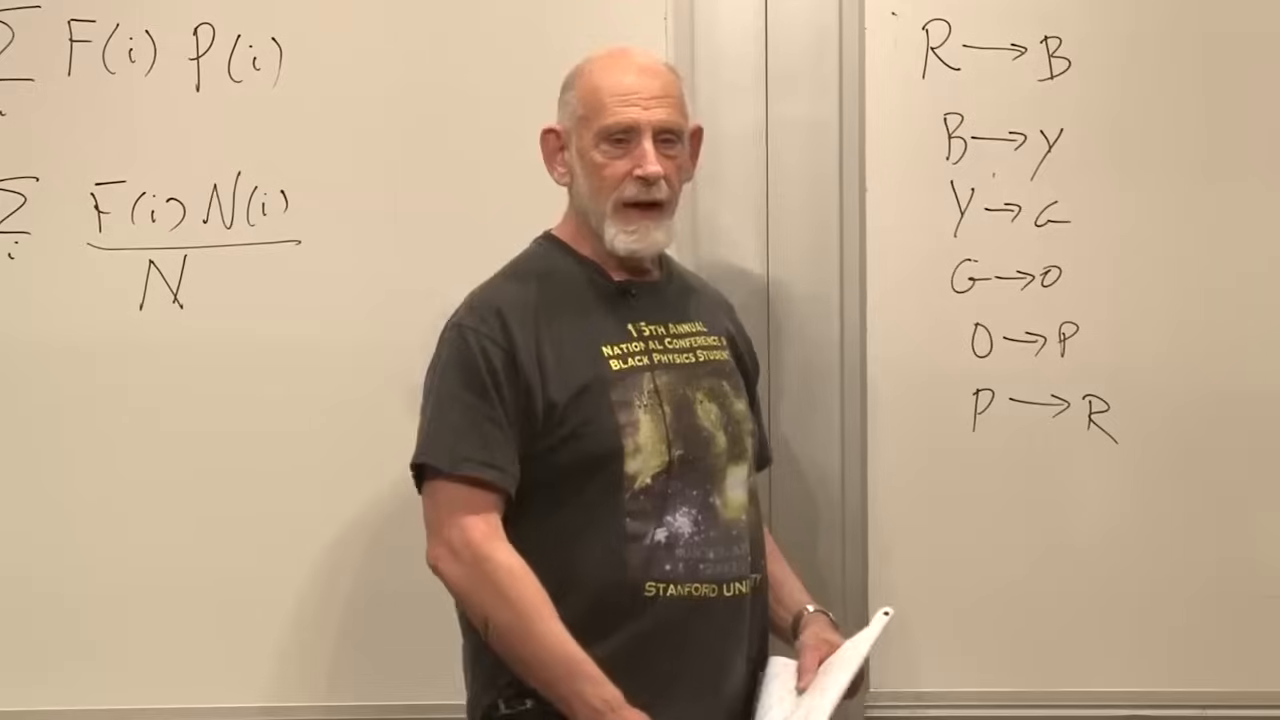
\includegraphics[width=0.92\textwidth]{lecture_01_figure_02.png}
\caption{Las fórmulas de los valores esperados permanecen en la pizarra de la izquierda, mientras que en la de la derecha se enumeran las seis actualizaciones deterministas de color.}
\lectureframe{00:26:28}
\end{figure}

La lista de la pizarra se entiende mejor si se representa como un ciclo dirigido:
\begin{figure}[htbp]
\centering
\begin{tikzpicture}[
  >=Latex,
  state/.style={draw,circle,minimum size=8mm,inner sep=1pt}
]
\node[state] (R) at (90:2.2) {$R$};
\node[state] (B) at (30:2.2) {$B$};
\node[state] (Y) at (-30:2.2) {$Y$};
\node[state] (G) at (-90:2.2) {$G$};
\node[state] (O) at (-150:2.2) {$O$};
\node[state] (P) at (150:2.2) {$P$};
\draw[->] (R) -- (B);
\draw[->] (B) -- (Y);
\draw[->] (Y) -- (G);
\draw[->] (G) -- (O);
\draw[->] (O) -- (P);
\draw[->] (P) -- (R);
\end{tikzpicture}
\caption{Una única órbita de seis estados. Cada estado se visita una vez durante cada período.}
\label{fig:sm1-six-cycle}
\end{figure}

Supongamos que desconocemos el estado inicial y tomamos una instantánea en un instante también desconocido. Como todos los pasos duran lo mismo, el sistema pasa una sexta parte del período en cada color:
\begin{equation}
 p(R)=p(B)=p(Y)=p(G)=p(O)=p(P)=\frac16.
 \label{eq:sm1-uniform-cycle}
\end{equation}
La igualdad no se debe a la forma del objeto. Se debe a que el tiempo transcurrido en cada estado es el mismo.

Podemos reordenar las flechas y obtener una ley microscópica distinta que siga formando un único ciclo de seis estados. La secuencia detallada cambia, pero la probabilidad de observar una instantánea sigue siendo \(1/6\), porque cada estado continúa apareciendo una vez por período. Por tanto, esta predicción no requiere conocer el punto de partida ni el orden detallado. Solo requiere la estructura de la órbita y el mismo tiempo para cada actualización.

\begin{classroomqa}
\classquestion{Si el objeto no es simétrico, ¿en qué sentido es
legítimo asignar a cada color una probabilidad \(1/6\)?}
\lecturerresponse{La asignación es dinámica, no geométrica. Una
instantánea tomada en una fase desconocida de una órbita de seis pasos muestrea seis intervalos de tiempo iguales. La equivalencia relevante es la de las posiciones en la órbita, no la de las caras del objeto. Si los tiempos de permanencia fueran distintos, las probabilidades también serían distintas.
\lecturetimestamp{00:27:11--00:29:49}}
\end{classroomqa}

\section{Ciclos desconectados y magnitudes conservadas}

Una ley determinista no tiene por qué situar todos los estados en una única órbita. Consideremos dos ciclos desconectados,
\begin{equation}
 R\longrightarrow B\longrightarrow G\longrightarrow R,
 \qquad
 P\longrightarrow Y\longrightarrow O\longrightarrow P.
 \label{eq:sm1-two-cycles}
\end{equation}
Si sabemos que el sistema está en el primer ciclo, entonces
\begin{equation}
 \begin{aligned}
 p(R)=p(B)=p(G)&=\frac13,\\
 p(P)=p(Y)=p(O)&=0.
 \end{aligned}
\end{equation}
Saber que está en el segundo ciclo invierte estas asignaciones.

El caso más general requiere pesos previos. Etiquetemos los ciclos con \(+1\) y \(-1\), y sean sus probabilidades \(p_+\) y \(p_-\), con
\begin{equation}
 p_++p_-=1.
\end{equation}
Entonces
\begin{align}
 p(R)=p(B)=p(G)&=\frac{p_+}{3},\\
 p(P)=p(Y)=p(O)&=\frac{p_-}{3}.
 \label{eq:sm1-sector-weights}
\end{align}
Los factores \(1/3\) se deben al movimiento dentro de cada ciclo. Los números \(p_+\) y \(p_-\) no. Deben provenir de información adicional, quizá de otro experimento o de otro sistema que seleccione el sector inicial.

Las etiquetas \(+1\) y \(-1\) definen una magnitud conservada: una vez que el sistema empieza en un ciclo, la ley de actualización nunca lo lleva al otro. Podemos llamar energía a esa magnitud o darle un nombre provisional como \emph{zilch}. El nombre es secundario. La conservación significa que el espacio de estados queda dividido en regiones que la dinámica no puede atravesar.

Los ciclos no tienen por qué contener el mismo número de estados. Una órbita de cuatro estados y otra de dos siguen definiendo dos sectores conservados. El muestreo con tiempos iguales da entonces \(1/4\) dentro del primero y \(1/2\) dentro del segundo, multiplicadas en ambos casos por la probabilidad previa de ese sector. La mecánica estadística debe responder a dos preguntas lógicamente distintas:
\begin{enumerate}
\item Dado un sector conservado, ¿cuánto tiempo pasa la dinámica en sus estados?
\item ¿Qué probabilidad debe asignarse al propio sector conservado?
\end{enumerate}

\begin{classroomqa}
\audiencequestion{¿Suponemos que todos los estados de un mismo
sector conservado reciben la misma probabilidad?}
\lecturerresponse{En las leyes discretas sencillas que se muestran aquí, sí, porque cada estado dura el mismo intervalo de tiempo y el movimiento es determinista. La incertidumbre está en la fase inicial de la órbita. Un detector con resolución temporal de milisegundos no puede resolver actualizaciones de microsegundos, aunque una instantánea lo bastante rápida aún puede identificar el estado que captó. En un sistema más general, deben tenerse en cuenta explícitamente los tiempos de permanencia desiguales.
\lecturetimestamp{00:36:16--00:37:17}}
\end{classroomqa}

\begin{classroomqa}
\audiencequestion{Si se toman dos instantáneas y la primera identifica un
ciclo, ¿debería la segunda identificar el mismo ciclo?}
\lecturerresponse{Sí. Eso es precisamente lo que significa la conservación. Una vez que una medición determina el valor de la magnitud conservada, las probabilidades futuras pueden condicionarse a ese valor, y a los estados del otro sector se les asigna probabilidad cero.
\lecturetimestamp{00:37:18--00:37:45}}
\end{classroomqa}

\subsection{Energía compartida entre dos sistemas}

Ahora reemplacemos la etiqueta abstracta por la energía. Una caja aislada es un sistema cerrado y tiene una energía conservada. Dos cajas aisladas tienen energías conservadas por separado porque no interactúan. Conectémoslas mediante un pasaje estrecho que permita el flujo de energía: las energías por separado pueden cambiar, pero la energía total permanece constante.

\begin{figure}[htbp]
\centering
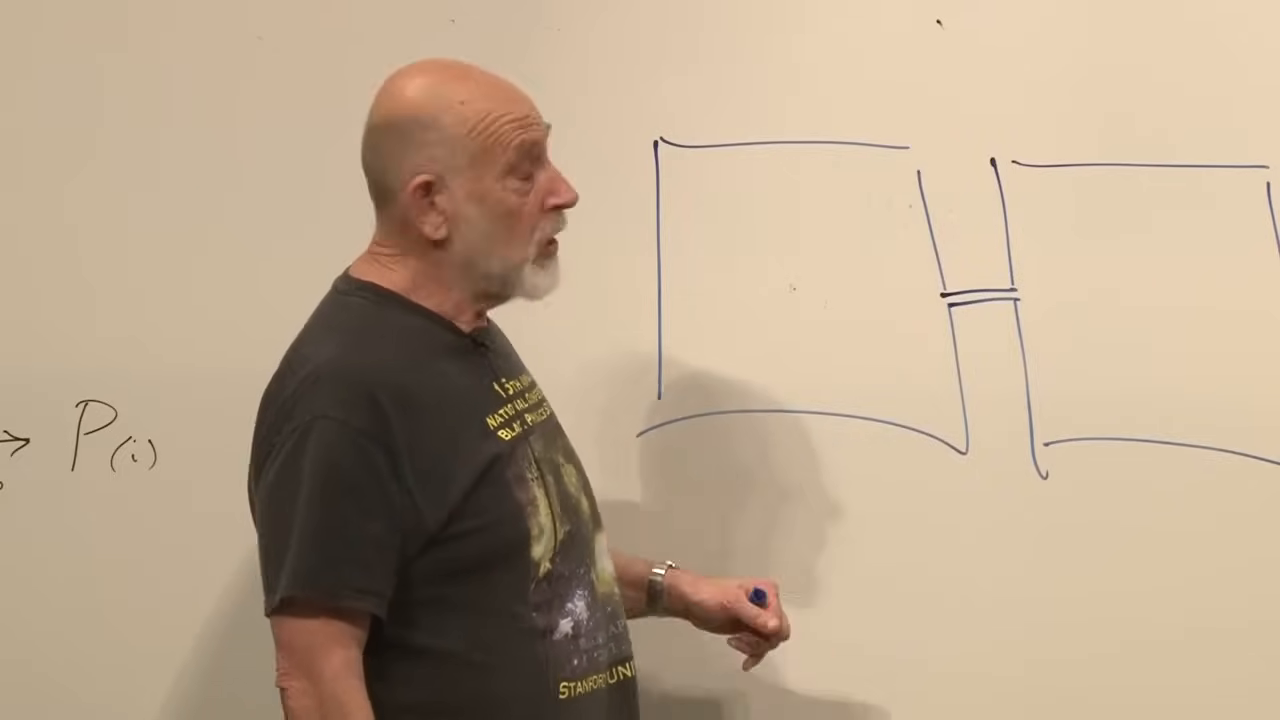
\includegraphics[width=0.92\textwidth]{lecture_01_figure_03.png}
\caption{Dos subsistemas conectados por un canal estrecho por el que puede pasar energía.}
\lectureframe{00:39:19}
\end{figure}

\begin{figure}[htbp]
\centering
\begin{tikzpicture}[>=Latex]
\draw[thick,rounded corners=4pt] (-4,1.8) rectangle (-0.7,-1.5);
\draw[thick,rounded corners=4pt] (0.7,1.5) rectangle (4,-1.8);
\draw[thick] (-0.7,0.45) -- (0.7,0.45);
\draw[thick] (-0.7,-0.35) -- (0.7,-0.35);
\draw[<->,very thick] (-0.45,0.05) -- (0.45,0.05);
\node at (-2.35,0.15) {subsystem \(1\)};
\node at (2.35,-0.15) {subsystem \(2\)};
\node[above] at (0,0.5) {energy exchange};
\end{tikzpicture}
\caption{Una vez abierta la conexión, solo se conserva \(E_1+E_2\). El reparto de energía se convierte en un problema de probabilidad.}
\label{fig:sm1-connected-systems}
\end{figure}

Dada una energía total, podemos preguntar cuál es la probabilidad de que el subsistema \(1\) tenga \(E_1\) y el subsistema \(2\) tenga el resto. Si las cajas son iguales, deberían tener la misma energía en promedio, pero el promedio no describe toda la distribución. Por tanto, una manera de determinar las probabilidades de un subsistema consiste en incluirlo en un sistema cerrado mayor cuya ley de conservación aporte la información que falta. Esta construcción reaparecerá a lo largo de la mecánica estadística.

\section{Leyes buenas, leyes malas y la ley menos uno}

No toda regla determinista de actualización es admisible como ley fundamental. Consideremos la aplicación
\begin{equation}
 \begin{aligned}
 R&\mapsto R,& B&\mapsto R,& Y&\mapsto R,\\
 G&\mapsto R,& O&\mapsto R,& P&\mapsto R.
 \end{aligned}
 \label{eq:sm1-all-to-red}
\end{equation}
Predice el futuro a la perfección: tras un paso, el estado es rojo. Falla en la dirección opuesta. Una vez que el sistema está en rojo, nada permite saber si llegó allí desde azul, amarillo, verde, naranja, morado o desde el propio rojo.

\begin{figure}[htbp]
\centering
\begin{tikzpicture}[
  >=Latex,
  state/.style={draw,circle,minimum size=8mm,inner sep=1pt}
]
\node[state,fill=red!12] (R) at (0,0) {$R$};
\node[state] (B) at (-3,1.6) {$B$};
\node[state] (Y) at (-3,0) {$Y$};
\node[state] (G) at (-3,-1.6) {$G$};
\node[state] (O) at (3,1.6) {$O$};
\node[state] (P) at (3,-1.6) {$P$};
\draw[->] (B) -- (R);
\draw[->] (Y) -- (R);
\draw[->] (G) -- (R);
\draw[->] (O) -- (R);
\draw[->] (P) -- (R);
\draw[->,loop above] (R) to (R);
\end{tikzpicture}
\caption{Una ley de muchos a uno predice el estado siguiente, pero borra las distinciones entre los posibles estados anteriores.}
\label{fig:sm1-bad-law}
\end{figure}

En cambio, un ciclo cerrado conserva el registro. Si conocemos el tiempo transcurrido, podemos hacer evolucionar el estado hacia adelante o hacia atrás, incluso después de muchos miles de períodos. La ley conserva las distinciones entre las condiciones iniciales. Susskind denomina a este requisito la \emph{ley menos uno de la física}: la información no se pierde de forma fundamental.

Para un espacio de estados discreto y finito, el criterio diagramático es sencillo:
\begin{quote}
Toda ley buena asigna exactamente una flecha saliente y exactamente una flecha entrante a cada estado.
\end{quote}
La flecha saliente determina el futuro; la entrante reconstruye el pasado. Matemáticamente, la actualización es una permutación de los estados.

\subsection{La fricción solo es un contraejemplo aparente}

La versión continua correspondiente es el teorema de Liouville. La fricción parece contradecirlo. Deslicemos una goma de borrar sobre una mesa: dondequiera que empiece, acaba deteniéndose. Una ecuación esquemática de arrastre es
\begin{equation}
 m\ddot x=-\gamma\dot x,
 \qquad \gamma>0.
 \label{eq:sm1-drag}
\end{equation}
Su velocidad decae exponencialmente. Si esta fuera la ley fundamental de todas las partículas de una habitación sellada, todo movimiento se extinguiría, la temperatura caería a cero y muchos estados iniciales convergerían en un único estado final. Fallaría la conservación de la energía, desaparecería información y disminuiría el desorden. Sería la versión continua de que todo se vuelve rojo.

La fricción real no funciona así. La goma calienta la mesa, a sí misma y al entorno. Las posiciones y los momentos microscópicos registran las distinciones que se pierden en el movimiento visible. La fricción es una ecuación efectiva para un subsistema, una vez omitidos los grados de libertad no observados; no es una ley fundamental disipativa para el sistema cerrado completo.

\begin{classroomqa}
\classquestion{¿Qué representa la ecuación diferencial
\(m\ddot x=-\gamma\dot x\) y por qué no es una ley fundamental para un
sistema cerrado?}
\lecturerresponse{Representa el arrastre viscoso. Por sí sola, hace que todas las velocidades tiendan a cero, lo que enfriaría un gas hasta cero cualquiera que fuera su temperatura inicial. En una descripción real de un sistema cerrado, la energía mecánica y la información perdidas pasan a los grados de libertad microscópicos. La ecuación de arrastre solo es fiable una vez que se han omitido esas variables.
\lecturetimestamp{00:44:40--00:48:56}}
\end{classroomqa}

\section{Estados ocupados y primera entropía}

La conservación de la información tiene un enunciado probabilístico equivalente. Supongamos que se asigna la misma probabilidad a \(M\) de los \(N\) estados,
\begin{equation}
 p_i=
 \begin{cases}
 1/M, & i\text{ in the occupied set},\\
 0, & i\text{ outside it}.
 \end{cases}
 \label{eq:sm1-uniform-occupied}
\end{equation}
Una actualización que conserva la información puede reorganizar los estados ocupados, pero no puede fusionarlos. En cualquier tiempo posterior siguen habiendo \(M\) estados con probabilidad \(1/M\). En cambio, la aplicación no adecuada \eqref{eq:sm1-all-to-red} puede hacer que muchos estados ocupados colapsen en uno solo.

El número \(M\) mide la ignorancia. Si \(M=N\), todos los estados son posibles y nuestra ignorancia es máxima. Si \(M=1\), se conoce exactamente el estado microscópico. Por tanto, la primera definición de entropía es
\begin{equation}
 S=\log M.
 \label{eq:sm1-entropy-logm}
\end{equation}
De ahí se obtiene
\begin{equation}
 S_{\max}=\log N,
 \qquad
 S_{\min}=0.
\end{equation}
Si el espacio de estados es infinito, puede no haber una cota superior finita.

En este desarrollo, la entropía aparece antes que la temperatura e incluso antes del enunciado formal de la conservación de la energía. En ese sentido, es más primitiva. Sin embargo, no es una propiedad exclusiva del sistema mecánico. Depende conjuntamente del sistema y de la distribución de probabilidad que representa lo que se conoce. Observadores con información distinta pueden asignar entropías distintas al mismo sistema mecánico.

Bajo una evolución microscópica exacta, los estados ocupados solo se reorganizan, por lo que esta entropía de grano fino se conserva. En la práctica, perdemos la información temporal, descartamos correlaciones y no conseguimos seguir la pista a cantidades enormes de variables. Entonces nuestra distribución de probabilidad se extiende sobre más alternativas y aumenta la entropía asignada a la descripción gruesa. Las ecuaciones no tienen por qué destruir la información para que nuestra descripción utilizable la pierda.

\begin{classroomqa}
\classquestion{¿Cuál es la entropía máxima posible de un sistema finito
con \(N\) estados?}
\lecturerresponse{Es \(\log N\), y se alcanza cuando los \(N\) estados tienen
la misma probabilidad. La entropía mínima es cero y se alcanza cuando un estado tiene probabilidad uno. Por tanto, la entropía mide tanto el estado del conocimiento como el espacio de estados disponible.
\lecturetimestamp{00:56:46--00:58:19}}
\end{classroomqa}

\section{Flujo de Liouville en el espacio de fases continuo}

Para partículas con posiciones y momentos continuos, un estado microscópico es un punto del espacio de fases. Escribimos las coordenadas como \(q_a\) y sus momentos conjugados como \(p_a\). Con muchas partículas hay un número enorme de ejes; un dibujo bidimensional con un \(q\) y un \(p\) es solo una representación esquemática. El espacio de fases es de dimensión par porque cada coordenada tiene un momento asociado.

Supongamos que nuestro conocimiento se representa mediante una región \(\Omega_0\): la densidad de probabilidad es uniforme dentro de ella y nula fuera. Por ejemplo, saber que todas las partículas están en la habitación restringe las coordenadas de posición, mientras que imponer límites a sus velocidades restringe las coordenadas de momento.

La evolución hamiltoniana hace que cada punto del espacio de fases siga una trayectoria. Los puntos próximos se transforman en puntos próximos, y la región ocupada fluye como una porción de fluido incompresible:
\begin{figure}[htbp]
\centering
\begin{tikzpicture}[>=Latex,scale=0.95]
\draw[->] (-4.2,0) -- (4.3,0) node[right] {$q$};
\draw[->] (-3.7,-2.2) -- (-3.7,2.4) node[above] {$p$};
\draw[fill=blue!12,thick]
  (-3.0,-0.5) .. controls (-2.7,1.0) and (-1.3,1.2) .. (-0.9,0.1)
  .. controls (-0.6,-1.0) and (-2.2,-1.4) .. cycle;
\node at (-1.9,0.0) {$\Omega_0$};
\draw[->,very thick] (-0.3,0.2) -- (0.8,0.2);
\draw[fill=orange!15,thick]
  (1.2,-1.1) .. controls (1.5,0.3) and (2.3,1.8) .. (3.2,1.1)
  .. controls (3.6,0.7) and (2.8,-0.4) .. (2.5,-1.5)
  .. controls (2.1,-1.8) and (1.5,-1.6) .. cycle;
\node at (2.35,0.1) {$\Omega_t$};
\end{tikzpicture}
\caption{El flujo hamiltoniano puede estirar y deformar por cizallamiento una región ocupada del espacio de fases, pero conserva su volumen.}
\label{fig:sm1-liouville-flow}
\end{figure}

El teorema de Liouville establece que
\begin{equation}
 \operatorname{Vol}(\Omega_t)
 =
 \operatorname{Vol}(\Omega_0).
 \label{eq:sm1-liouville-volume}
\end{equation}
Si la densidad inicial es uniforme en \(\Omega_0\), la densidad transportada es uniforme en \(\Omega_t\). Este es el análogo continuo de conservar el número y los pesos de los estados discretos ocupados.

El teorema también resuelve geométricamente el enigma de la fricción. Si solo observamos el momento visible de la goma, una nube de posibilidades parece contraerse hacia \(p=0\). En el espacio de fases completo, la nube se extiende por las posiciones y los momentos de las moléculas de la goma y de la mesa. Una proyección puede contraerse mientras el volumen total de alta dimensión permanece constante.

\begin{classroomqa}
\classquestion{Si todas las trayectorias visibles se acercan al reposo, ¿se ha
contraído la región ocupada del espacio de fases hasta el eje \(p=0\)?}
\lecturerresponse{Solo en la proyección reducida. El sistema completo
contiene las variables microscópicas de la mesa, la goma y el entorno. A medida que se estrecha el intervalo del momento visible, la distribución se extiende por esas direcciones ocultas. El teorema de Liouville se aplica al espacio de fases completo del sistema cerrado, no a un conjunto incompleto de variables macroscópicas.
\lecturetimestamp{01:04:37--01:06:29}}
\end{classroomqa}

\section{De la ley menos uno a la primera ley}

\subsection{Breve introducción a la ley cero}

Antes de enunciar la primera ley, conviene nombrar la ley cero. Aún no hemos definido el equilibrio térmico, así que por ahora la ley solo expresa una propiedad estructural:
\begin{quote}
Si el sistema \(A\) está en equilibrio térmico con \(B\), y \(B\) está en equilibrio térmico con \(C\), entonces \(A\) está en equilibrio térmico con \(C\).
\end{quote}
Esta transitividad permitirá definir la temperatura más adelante. Por ahora, la dejamos a un lado.

\subsection{Conservación de la energía}

La primera ley para un sistema cerrado es, sencillamente,
\begin{equation}
 \frac{dE}{dt}=0.
 \label{eq:sm1-first-law}
\end{equation}
Su forma compacta oculta su alcance. La energía es una magnitud conservada, y más adelante el término energía adquirirá un contenido termodinámico más amplio.

Si un sistema cerrado consta de dos partes y sus energías son aditivas,
\begin{equation}
 E=E_1+E_2,
\end{equation}
entonces
\begin{equation}
 \frac{dE_1}{dt}+\frac{dE_2}{dt}=0,
 \qquad\text{or}\qquad
 \frac{dE_1}{dt}=-\frac{dE_2}{dt}.
 \label{eq:sm1-energy-exchange}
\end{equation}
La segunda forma hace explícito el intercambio: la energía que pierde un subsistema la gana el otro.

La hipótesis de aditividad exige cuidado. Dos partículas que gravitan tienen energías cinéticas individuales, pero su interacción aporta una energía potencial que corresponde al par. La energía total se conserva, aunque no pueda escribirse exactamente como la energía de un cuerpo más la del otro.

En termodinámica suele ser posible una aproximación aditiva excelente, porque la energía macroscópica escala con el volumen, mientras que la energía de interacción de corto alcance entre piezas grandes vecinas depende principalmente del área de contacto. Dividamos una mesa grande en bloques: la energía interna de cada bloque es un efecto de volumen, mientras que el acoplamiento entre bloques adyacentes es un efecto superficial. En bloques grandes, este último es comparativamente pequeño. La ecuación \eqref{eq:sm1-first-law} es exacta para el conjunto cerrado; la forma para los subsistemas, \eqref{eq:sm1-energy-exchange}, supone que la energía de interacción es despreciable.

\begin{classroomqa}
\audiencequestion{¿La normalización \(\sum_i p_i=1\) también supone que los
resultados enumerados son mutuamente excluyentes?}
\lecturerresponse{Sí. Las etiquetas de estado se definen de modo que las alternativas no se solapen: si el dado está en el estado amarillo, no está simultáneamente en el rojo. En el lenguaje corriente pueden mezclarse los colores, pero la partición de estados empleada en el cálculo de probabilidades debe constar de alternativas mutuamente excluyentes.
\lecturetimestamp{01:12:14--01:12:55}}
\end{classroomqa}

\section{Volvamos a la entropía}

Ahora la lección vuelve explícitamente a lo que quedó pendiente. La temperatura, aunque nos resulte familiar a través de los sentidos, es una magnitud derivada. La entropía y la energía deben estar establecidas antes de poder definirla con claridad.

\subsection{Distribuciones de probabilidad generales}

La definición particular \(S=\log M\) se aplica cuando \(M\) estados tienen la misma probabilidad y todos los demás tienen probabilidad cero. Una distribución general no tiene por qué ser rectangular. Sus pesos pueden variar de forma suave o irregular a lo largo de las etiquetas de estado.

\begin{figure}[htbp]
\centering
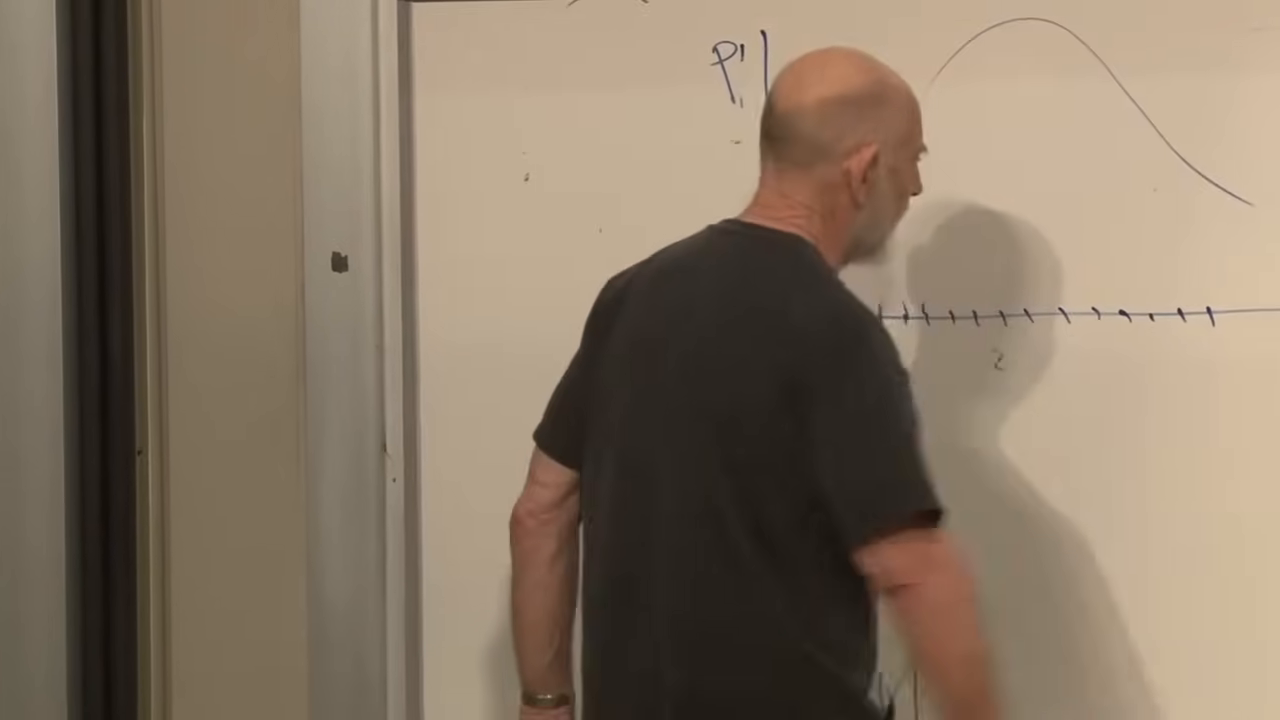
\includegraphics[width=0.92\textwidth]{lecture_01_figure_05.png}
\caption{Una distribución de probabilidad representada sobre etiquetas discretas de estado. Para la entropía, lo relevante es la dispersión, no la curva precisa.}
\lectureframe{01:14:40}
\end{figure}

\begin{figure}[htbp]
\centering
\resizebox{\linewidth}{!}{%
\begin{tikzpicture}[>=Latex,scale=0.93]
\draw[->] (-4.2,0) -- (4.4,0) node[right] {state label \(i\)};
\draw[->] (-4,0) -- (-4,3.2) node[above] {$p_i$};
\foreach \x in {-3.6,-3.1,...,3.6}
  \draw (\x,0.08) -- (\x,-0.08);
\draw[very thick]
  plot[smooth] coordinates {
  (-3.7,0.12) (-3.0,0.28) (-2.3,0.72) (-1.6,1.45)
  (-0.9,2.25) (-0.2,2.65) (0.5,2.28) (1.2,1.55)
  (1.9,0.88) (2.7,0.38) (3.5,0.14)};
\draw (-1.8,-0.18) -- (-1.8,-0.5);
\draw (1.8,-0.18) -- (1.8,-0.5);
\draw[<->] (-1.8,-0.46) -- (1.8,-0.46);
\node at (0,-0.82) {effective spread};
\end{tikzpicture}
}
\caption{Una distribución estrecha conlleva menos incertidumbre que una amplia. La entropía debe medir la distribución en su conjunto.}
\label{fig:sm1-probability-spread}
\end{figure}

La definición general es
\begin{equation}
 S=-\sum_i p_i\log p_i.
 \label{eq:sm1-shannon-entropy}
\end{equation}
Usando \eqref{eq:sm1-expectation}, se obtiene
\begin{equation}
 S=-\langle\log p\rangle.
\end{equation}
El signo menos compensa el hecho de que \(\log p_i<0\) cuando
\(0<p_i<1\).

\subsection{Recuperación del resultado uniforme}

Debemos comprobar que la fórmula general reproduce la primera definición.
Para un estado desocupado, \(p_i=0\) mientras que \(\log p_i\) diverge. El producto tiene el siguiente valor límite bien definido:
\begin{equation}
 \lim_{p\to0^+}p\log p=0.
 \label{eq:sm1-plogp-limit}
\end{equation}
Por tanto, los estados con probabilidad cero no contribuyen.

\begin{classroomqa}
\audiencequestion{Si \(p_i=0\), ¿el término realmente se anula? El logaritmo de cero es menos infinito.}
\lecturerresponse{El término se define mediante el límite
\(\lim_{p\to0^+}p\log p\), que es cero. El factor \(p\) tiende a cero más rápido de lo que diverge el logaritmo. Por tanto, los estados arbitrariamente improbables aportan cantidades arbitrariamente pequeñas, y un estado exactamente imposible no aporta nada.
\lecturetimestamp{01:18:27--01:19:46}}
\end{classroomqa}

Para cada uno de los \(M\) estados ocupados, \(p_i=1/M\). Por tanto,
\begin{align}
 S
 &=-\sum_{\mathrm{occupied}\ i}
 \frac1M\log\!\left(\frac1M\right)\\
 &=-M\frac1M\log\!\left(\frac1M\right)\\
 &=-\log\!\left(\frac1M\right)
 =\log M.
 \label{eq:sm1-entropy-check}
\end{align}
La expresión general coincide exactamente con la particular. Una distribución más amplia asigna un peso apreciable a más alternativas y, por tanto, tiene mayor entropía; una distribución más estrecha tiene menor entropía.

\begin{figure}[htbp]
\centering
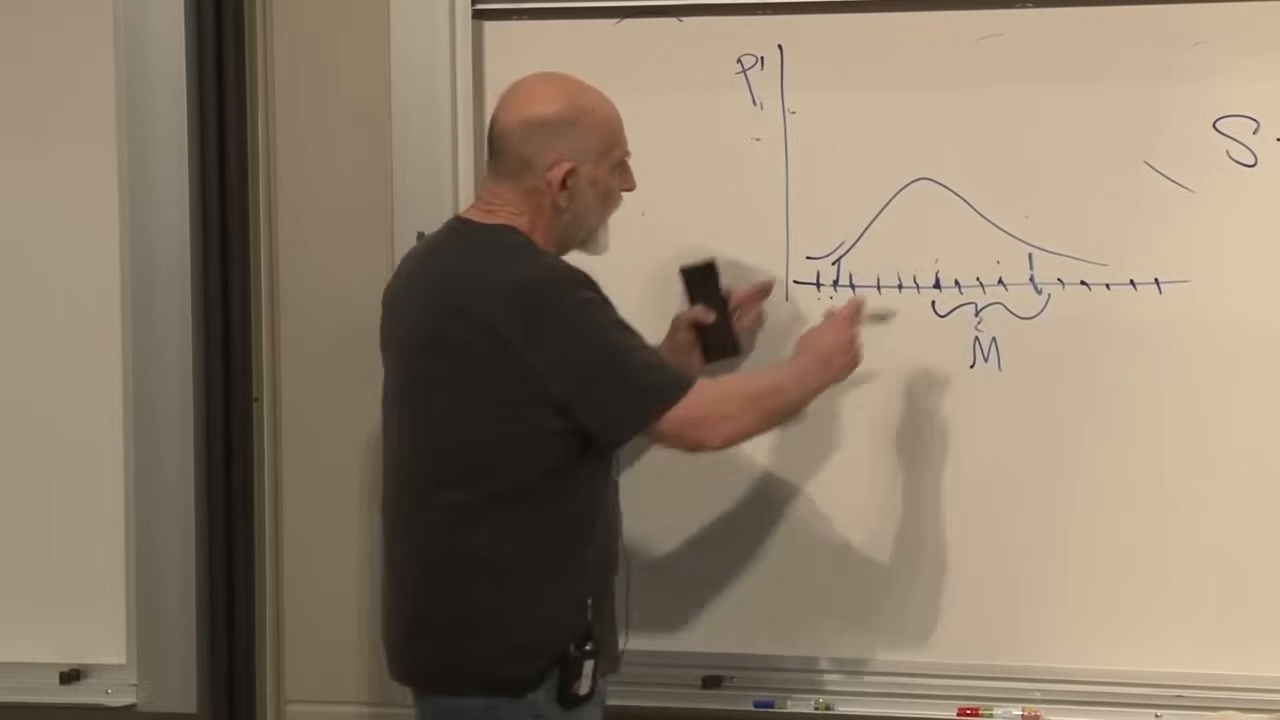
\includegraphics[width=0.92\textwidth]{lecture_01_figure_06.png}
\caption{La anchura indicada \(M\) resalta la relación entre la dispersión de las probabilidades significativas y la entropía.}
\lectureframe{01:16:42}
\end{figure}

La entropía corresponde a una distribución de probabilidad sobre el espacio de estados. No es una magnitud observable aislada, como la energía o el momento de un microestado. Un estado exacto puede representarse mediante una distribución concentrada en ese estado y, en tal caso, tiene entropía cero; sin embargo, la entropía cambia cuando cambia nuestro estado de conocimiento.

\section{Monedas, bits y recuento explícito}

Sea \(n\) el número de monedas. El número de configuraciones microscópicas es
\begin{equation}
 N=2^n.
 \label{eq:sm1-coin-state-count}
\end{equation}
Si no se sabe nada sobre las monedas, las \(2^n\) configuraciones son igualmente probables, y
\begin{equation}
 S_{\max}=\log(2^n)=n\log2.
 \label{eq:sm1-coin-max-entropy}
\end{equation}
La entropía es aditiva respecto al número de monedas independientes.

Con logaritmos en base \(2\), un sistema de dos estados completamente desconocido tiene una entropía de un bit. Con logaritmos naturales, su entropía es \(\log2\). La unidad es convencional; el orden subyacente y la aditividad no cambian.

En el otro extremo, si se conoce el resultado de cada moneda, una única configuración tiene probabilidad uno:
\begin{equation}
 S=0.
\end{equation}
Cuanto mayor es el conocimiento, menor es la entropía.

Supongamos ahora que exactamente una de las \(n\) monedas muestra cruz, todas las demás muestran cara y se desconoce la posición de la cruz. Hay \(n\) configuraciones igualmente probables, una por cada posición posible de la cruz, así que
\begin{equation}
 S=\log n.
 \label{eq:sm1-one-tail-entropy}
\end{equation}
En general, esto no es un múltiplo entero de \(\log2\). El bit es una unidad conveniente; no implica que toda entropía se presente en incrementos de bits enteros.

\begin{classroomqa}
\audiencequestion{¿Aparece \(\log2\) solo porque cada moneda tiene dos estados posibles? ¿Un elemento con tres estados daría \(\log3\)?}
\lecturerresponse{Exactamente. Un elemento con \(k\) estados posibles, todos igualmente desconocidos, aporta \(\log k\). Los interruptores binarios son especialmente convenientes en los ordenadores porque los interruptores físicos realizan de manera natural dos estados estables y porque dos es el menor entero no trivial.
\lecturetimestamp{01:29:55--01:30:48}}
\end{classroomqa}

\begin{classroomqa}
\audiencequestion{¿En qué base está definido el logaritmo?}
\lecturerresponse{En estas fórmulas de física, \(\log\) denota el logaritmo natural. Los teóricos de la información suelen usar la base \(2\), de modo que la entropía se mide directamente en bits. Cambiar la base multiplica todas las entropías por un mismo factor de conversión y no altera ninguna conclusión física.
\lecturetimestamp{01:30:49--01:32:06}}
\end{classroomqa}

\section{Entropía en el espacio de fases continuo}

Volvamos a un espacio de fases clásico \(\Gamma\). Si la densidad de probabilidad es uniforme en una región de volumen \(V_\Gamma\) y nula fuera de ella, el análogo de contar \(M\) estados igualmente probables es
\begin{equation}
 S=\log\!\left(\frac{V_\Gamma}{V_0}\right).
 \label{eq:sm1-continuous-uniform}
\end{equation}
Aquí \(V_\Gamma\) es el volumen en el espacio completo de coordenadas y momentos, de alta dimensión, no el volumen espacial ordinario. El volumen fijo \(V_0\) es una celda de referencia del espacio de fases que hace adimensional el argumento del logaritmo. Si se toma \(V_0=1\), se obtiene la forma abreviada \(S=\log V_\Gamma\) utilizada en la pizarra.

Para una densidad de probabilidad general \(P(q,p)\), la suma discreta se convierte en una integral sobre el espacio de fases. La normalización es
\begin{equation}
 \int_\Gamma d\Gamma\,P(q,p)=1,
 \label{eq:sm1-continuous-normalization}
\end{equation}
y la entropía es
\begin{equation}
 S=-\int_\Gamma d\Gamma\,
 P(q,p)\log\!\bigl[P(q,p)V_0\bigr].
 \label{eq:sm1-continuous-entropy}
\end{equation}
La densidad es la probabilidad por celda del espacio de fases. Conceptualmente, \eqref{eq:sm1-continuous-entropy} sigue midiendo cuán ampliamente se distribuye la probabilidad; para una distribución uniforme, se reduce al logaritmo del volumen ocupado medido en unidades de la celda de referencia. Cambiar esa celda fija desplaza todas las entropías continuas en la misma constante aditiva y deja inalteradas las diferencias de entropía.

\begin{classroomqa}
\audiencequestion{¿Por qué cambió el símbolo de coordenada de \(x\) a \(q\)?}
\lecturerresponse{No hay ningún cambio físico. En mecánica clásica se suele usar \(x\) o \(q\) para las coordenadas y \(p\) para los momentos conjugados. El cambio de notación fue solo un desliz; la construcción del espacio de fases es la misma.
\lecturetimestamp{01:37:10--01:37:39}}
\end{classroomqa}

La temperatura y la distribución de Boltzmann se dejan deliberadamente para más adelante. El siguiente paso será definir el equilibrio térmico y, después, identificar su distribución de probabilidad.

\section{Preguntas sobre correlación, aditividad e información}

\subsection{La correlación significa que una medición modifica otra distribución}

La ignorancia completa sobre monedas independientes asigna la misma probabilidad a todas las configuraciones. Medir una moneda no nos dice nada sobre ninguna de las otras. Sus distribuciones no cambian.

El conjunto de casos con una sola cruz es distinto. Si una moneda medida muestra cruz, todas las demás muestran necesariamente cara. Si la moneda medida muestra cara, la única cruz tiene que estar entre las \(n-1\) monedas restantes, así que cada posición restante tiene probabilidad condicionada
\begin{equation}
\begin{aligned}
 p(&\text{tail at a specified remaining position}\\
   &\mid\text{measured head})=\frac{1}{n-1}.
\end{aligned}
 \label{eq:sm1-conditional-tail}
\end{equation}
Esto es correlación: conocer una variable modifica la distribución de probabilidad asignada a otra.

\begin{classroomqa}
\audiencequestion{¿Se supuso que las monedas eran independientes en los ejemplos de entropía?}
\lecturerresponse{Solo cuando la ignorancia completa se representó asignando probabilidades iguales a las \(2^n\) configuraciones. En ese caso, medir una moneda no modifica las distribuciones de las demás. El ejemplo de una sola cruz tiene correlaciones explícitas: una medición actualiza lo que es posible en las otras posiciones. La información especificada determina qué distribución de probabilidad se utiliza.
\lecturetimestamp{01:38:43--01:41:58}}
\end{classroomqa}

El ejemplo del ciclo desconectado tiene la misma estructura lógica. Medir la etiqueta conservada \(+1\) o \(-1\) restringe todos los estados posteriores a un único sector. Condicionar por la información conservada cambia la distribución admisible.

La entropía es aditiva para sistemas no correlacionados. Si
\begin{equation}
 p_{ij}=p_i^{(A)}p_j^{(B)},
\end{equation}
entonces
\begin{align}
 S_{AB}
 &=-\sum_{i,j}p_i^{(A)}p_j^{(B)}
 \log\!\left[p_i^{(A)}p_j^{(B)}\right]\\
 &=S_A+S_B.
 \label{eq:sm1-entropy-additivity}
\end{align}
Las correlaciones impiden esta factorización y reducen la incertidumbre independiente del par.

Como ejercicio, imaginemos una fila de variables binarias en la que un estado arriba hace que cada vecino tenga una probabilidad de tres cuartos de estar abajo. Medir un sitio cambia de inmediato lo que se sabe sobre los sitios cercanos. Esa distribución está correlacionada, y su entropía no puede calcularse sumando las entropías de cada sitio por separado sin tener en cuenta esas correlaciones.

\subsection{Boltzmann, Shannon e incertidumbre cuántica}

\begin{classroomqa}
\audiencequestion{¿Qué relación hay entre la antigua entropía termodinámica y la entropía informacional de Shannon?}
\lecturerresponse{En ambas aparece la misma forma funcional:
\(-\sum_i p_i\log p_i\). Shannon solía usar la base \(2\), mientras que los físicos suelen usar logaritmos naturales y recuperan la constante de Boltzmann cuando expresan la entropía en unidades termodinámicas. La diferencia matemática consiste solo en un factor de conversión fijo, aunque las preguntas físicas que determinan las probabilidades pueden ser muy distintas.
\lecturetimestamp{01:44:05--01:46:06}}
\end{classroomqa}

Para microestados igualmente probables, la fórmula termodinámica suele escribirse como
\begin{equation}
 S_{\mathrm{thermo}}=k_{\mathrm B}\log W,
 \label{eq:sm1-boltzmann-formula}
\end{equation}
donde \(W\) es el número de microestados accesibles. En unidades en las que \(k_{\mathrm B}=1\), esto es precisamente \(S=\log W\). La constante de Boltzmann convierte entre unidades de temperatura y unidades de energía; la escala microscópica natural de la temperatura es la energía.

\begin{classroomqa}
\audiencequestion{¿Es esta entropía simplemente otra forma del principio de incertidumbre de Heisenberg?}
\lecturerresponse{No. La entropía que estamos considerando mide la incertidumbre de una distribución de probabilidad sobre estados posibles. En lenguaje cuántico, es la incertidumbre de un estado mixto, no la incertidumbre intrínseca de una medición que puede persistir incluso en un estado puro. Hay que distinguir claramente ambas nociones.
\lecturetimestamp{01:46:07--01:47:31}}
\end{classroomqa}

\section{Lo que se ha establecido}

El punto de partida no fue la aleatoriedad de las leyes. La dinámica determinista, combinada con un conocimiento incompleto del estado inicial, ya produce probabilidades. Una sola órbita asigna pesos según el tiempo que pasa en cada estado; las órbitas desconectadas revelan cantidades conservadas y requieren asignar pesos previos entre sectores. Las leyes microscópicas admisibles preservan las distinciones, lo que, en un espacio de estados finito, significa que en cada estado hay una flecha entrante y una saliente; en mecánica continua, esto se expresa mediante el teorema de Liouville.

Esa estructura conduce primero a
\begin{equation}
 S=\log M
\end{equation}
para \(M\) estados ocupados igualmente probables; después, a
\begin{equation}
 S=-\sum_i p_i\log p_i,
\end{equation}
y, finalmente, a su integral sobre el espacio de fases. La entropía registra una distribución de probabilidad y, por tanto, un estado de conocimiento. La ley microscópica conserva la información de grano fino, aunque una descripción práctica de grano grueso deje de seguirla.

La conservación de la energía da lugar a la primera ley, mientras que la aditividad de las energías de los subsistemas requiere que la energía de interacción sea despreciable. La entropía es aditiva bajo una condición análoga: las probabilidades de los subsistemas no deben estar correlacionadas. Estas dos formas de aditividad preparan el siguiente paso, en el que el equilibrio térmico, la temperatura y la distribución de Boltzmann relacionarán la energía con la probabilidad.
